\section{Subsequence and the Bolzano-Weierstrass Theorem}
    \textbf{Definition 2.5.1.} Let $(a_n)$ be a sequence of real numbers, and let $n_1 < n_2 < n_3 < n_4 < \dots$ be an increasing sequence of natural numbers. Then the sequence 
    \begin{equation*}
        a_{n_1}, a_{n_2}, a_{n_3}, a_{n_4}, a_{n_5}, a_{n_6}, \dots
    \end{equation*}
    is called a \textit{subsequence} of $(a_n)$ and is denoted by $(a_{n_j})$, where $j \in \textbf{N}$ indexes the subsequence.
    \newline \indent
    The terms in a subsequence are in the same order as the original sequence, and repetitions are not allowed.
    \setcounter{theorem}{1}
    \begin{theorem}
        Subsequences of a convergent sequence converge to the same limit as the original sequence.
    \end{theorem}
    \begin{proof}
        TODO: Exercise 2.5.1
    \end{proof}
    \subsection*{The Bolzano–Weierstrass Theorem}
    \setcounter{theorem}{4}
    \begin{theorem}[The Bolzano–Weierstrass Theorem]
        Every bounded sequence contains a convergent subsequence.
    \end{theorem}
    \begin{proof}
        Let $(a_n)$ be a bounded sequence so that there exists $M > 0$ satisfying $|a_n| \leq M$ for all $n \in \textbf{N}$. Split $[-M, M]$ into $[-M, 0]$ and $[0, M]$. At least one of these intervals contain an infinite number of the points in the sequence $(a_n)$. Select a half for which this is the case and label that interval as $I_1$. Then, let $a_{n_1}$ be some point in the sequence $(a_n)$ satisfying $a_{n_1} \in I_1$.
        \begin{center}
            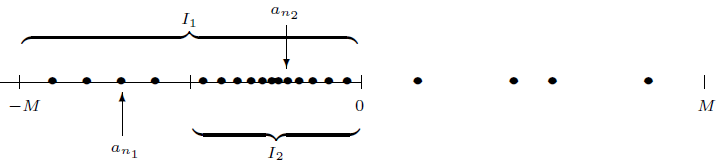
\includegraphics[width=250pt]{bolzano.png}
        \end{center}
        Next, we bisect $I_1$ into closed intervals of equal length, and let $I_2$ be a half that again contains an infinite number of points of the original sequence. Then choose an $a_{n_2}$ such that $n_2 > n_1$ and $a_{n_2} \in I_2$. In general, we construct the closed interval $I_k$ by taking a half of $I_{k-1}$ containing an infinite number of points of $(a_n)$ and then select $n_k > n_{k-1} > \dots > n_2 > n_1$ so that $a_{n_k+ \in I_k}$. The sets 
        \begin{equation*}
            I_1 \subseteq I_2 \subseteq I_3 \subseteq \dots
        \end{equation*}
        form a nested sequence of closed intervals, so by the Nested Interval Property there exists at least one point $x \in \textbf{R}$ contained in every $I_k$. Now, we will show that $(a_{n_k} \rightarrow x)$.
        \newline \indent
        Let $\epsilon > 0$. By construct, the length of $I_k$ is $M(1/2)^{k - 1}$ which converges to zero. Choose $N$ so that $k \geq N$ implies that the length of $I_k$ is less than $\epsilon$. Since $x$ and $a_{n_k}$ are both in $I_k$, it follows that $|a_{n_k} - x| < \epsilon$.
    \end{proof}